\documentclass[11pt,dvipsnames,usenames,aspectratio=169]{beamer}  % Add handout to options to disable overlays

% For more themes, color themes and font themes, see:
% http://deic.uab.es/~iblanes/beamer_gallery/index_by_theme.html
%
\mode<presentation>
{%
  \usetheme{CambridgeUS}    % or try default, Darmstadt, Warsaw, ...
  \usecolortheme{whale}     % or try albatross, beaver, crane, ...
  \usefonttheme{serif}          % or try default, structurebold, ...
  % \usefonttheme[onlymath]{serif}
  % \setbeamertemplate{navigation symbols}{}
  % \setbeamercovered{transparent}

  \setbeamercolor{title}{fg=white}
  \setbeamerfont{title}{series=\bfseries}
  \setbeamercolor{frametitle}{fg=black}
  \setbeamerfont{frametitle}{series=\bfseries}

  \setbeamercolor{section in head/foot}{fg=white}
  \setbeamerfont{section in head/foot}{series=\bfseries}
  \setbeamercolor{subsection in head/foot}{fg=white}
  \setbeamerfont{subsection in head/foot}{series=\bfseries}
  \setbeamercolor{author in head/foot}{fg=white}
  \setbeamerfont{author in head/foot}{series=\bfseries}
  \setbeamercolor{title in head/foot}{fg=white}
  \setbeamerfont{title in head/foot}{series=\bfseries}

  \setbeamercolor{block title}{use=structure,fg=white,bg=title in head/foot.bg}
  \setbeamerfont{block title}{series=\bfseries}
  \setbeamercolor{block body}{use=structure,fg=black,bg=black!1!white}
}

% Support graying out frame elements
\newcommand{\FrameOpague}{\setbeamercovered{again covered={\opaqueness<1->{40}}}}
% Transition slide
\newcommand{\transitionFrame}[1]{%
{%
  \begin{frame}[plain,noframenumbering]{}{} % the plain option removes the sidebar and header from the title page
    \setbeamertemplate{final page}[text]{\Large \textbf{#1}}
    \usebeamertemplate{final page}
  \end{frame}}
}

% \usepackage{hyperref}     % Loaded automatically by beamer
\usepackage{pgfplots}       % Used to generate embedded plots
\pgfplotsset{compat=1.13}

% Here's where the presentation starts, with the info for the title slide
\title[Towards Deep Robustness]{Towards Deep Learning Models Resistant to Adversarial Attacks~\cite{Madry:2017}}
\author[Madry et al]{%
  \href{mailto:madry@mit.edu}{Aleksander Madry}\inst{1}  % \textsuperscript{(\Letter)}
  \and
  \href{mailto:amakelov@mit.edu}{Aleksandar Makelov}\inst{1}  % \textsuperscript{(\Letter)}
  \and
  \href{mailto:ludwigs@mit.edu}{Ludwig Schmidt}\inst{1}  % \textsuperscript{(\Letter)}
  \and
  \href{mailto:tsipras@mit.edu}{Dimitris Tsipras}\inst{1}  % \textsuperscript{(\Letter)}
  \and
  \href{mailto:avladu@mit.edu}{Adrian Vladu}\inst{1}  % \textsuperscript{(\Letter)}
  % \href{mailto:lowd@cs.uoregon.edu}{Daniel Lowd}\inst{1}
}

\institute[MIT]{%
  \textsuperscript{1}\textbf{MIT -- CSAIL}\\
  % \texttt{{zayd, lowd}@ucsc.edu}
}
\date{\today}

\newcommand{\etal}{et~al.}
\newcommand{\elkan}{Elkan \&~Noto}

% Used for including standalone docs
\usepackage{standalone}

% Imported via UltiSnips
% Unbreakable dash:
%  Words hyphened with these dashes can also be broken at other positions than the dash
%    \-/ hyphen
%    \-- en-dash
%    \--- em-dash
%    extdash unbreakable dashes
%
%  No line breaks possible at the hyphen
%    \=/ hyphen
%    \== en-dash
%    \=== em-dash
\usepackage[shortcuts]{extdash}

% Imported via UltiSnips
\usepackage{color}
\newcommand{\colortext}[2]{{\color{#1} #2}}
\newcommand{\red}[1]{\colortext{red}{#1}}
\newcommand{\blue}[1]{\colortext{red}{#1}}
\newcommand{\green}[1]{\colortext{green}{#1}}

% Imported via UltiSnips
\usepackage{amsmath}
\DeclareMathOperator*{\argmax}{arg\,max}
\DeclareMathOperator*{\argmin}{arg\,min}
\DeclareMathOperator{\sgn}{sgn}
\usepackage{amsfonts}  % Used for \mathbb and \mathcal
\usepackage{amssymb}

% Imported via UltiSnips
\usepackage{mathtools} % for "\DeclarePairedDelimiter" macro
% \swapifbranches changes unstarred paired delimiters to starred and
% vice versa.  This means by default, paired delimiters have the star.
\usepackage{etoolbox}
\newcommand\swapifbranches[3]{#1{#3}{#2}}
\makeatletter
\MHInternalSyntaxOn
\patchcmd{\DeclarePairedDelimiter}{\@ifstar}{\swapifbranches\@ifstar}{}{}
\MHInternalSyntaxOff
\makeatother
% Place after swap to ensure swap star
\DeclarePairedDelimiter{\sbrack}{\lbrack}{\rbrack}
\DeclarePairedDelimiter{\floor}{\lfloor}{\rfloor}
\DeclarePairedDelimiter{\ceil}{\lceil}{\rceil}
\DeclarePairedDelimiter{\abs}{\lvert}{\rvert}
\DeclarePairedDelimiter{\norm}{\lVert}{\rVert}
\usepackage{bm}
\DeclarePairedDelimiterX\set[1]\lbrace\rbrace{#1}
\DeclarePairedDelimiterX\setbuild[2]\lbrace\rbrace{#1 \bm: #2}
\newcommand{\ints}[1]{{\sbrack{#1}}}
\newcommand{\func}[3]{{#1:#2\rightarrow#3}}
\newcommand{\defeq}{\stackrel{\mathclap{\mbox{\tiny def}}}{=}}

% Imported via UltiSnips
\usepackage{multirow}
\usepackage{booktabs}

% Imported via UltiSnips
\usepackage{tikz}
\usetikzlibrary{arrows,decorations.markings,shadows,positioning,calc,backgrounds,shapes}

\usepackage{graphicx}
\graphicspath{ {./img/} }

\newcommand{\distr}{\mathcal{D}}
\newcommand{\X}{x}
\newcommand{\y}{y}

\newcommand{\loss}{L}
\newcommand{\params}{\theta}

\newcommand{\sPerturb}{\mathcal{S}}

\renewcommand{\green}[1]{{\color{ForestGreen} #1}}


\begin{document}

\begin{frame}
  \titlepage
\end{frame}

\begin{frame}{Why is Adversarial Robustness Important?}
  Machine learning-based classifiers are increasing the center of \blue{security-critical systems}.
  \begin{itemize}
    \item \textit{Examples}: Autonomous cars, face recognition, \& malware detection
  \end{itemize}
  \vfill
  Training models can very effectively classify \green{benign} inputs
  \begin{itemize}
    \item \textit{Very small} changes to an input image can fool state of the art classifiers with \textit{high confidence}
    \item \textbf{Crucial Design Goal}: Resistance to \textit{adversarially chosen inputs}
  \end{itemize}
\end{frame}

\section{Background}
\begin{frame}{What is an Adversarial Example?}
  \onslide<+->{
    \begin{definition}
      \textit{\green{Adversarial Example}}: An input chosen/modified by an adversary that is almost indistinguishable from natural data but is (confidently) misclassified by the network.
    \end{definition}
  }

  \begin{columns}
    \begin{column}{0.23\textwidth}
      \onslide<+->{
        \begin{center}
          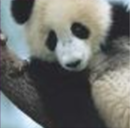
\includegraphics{adv_panda}

          \textbf{\blue{Prediction}}
          \\
          \textbf{Panda}
          \\
          55.7\% Confidence~\cite{Goodfellow:2014}
        \end{center}
      }
    \end{column}
    \onslide<+->{
      \begin{column}{0.05\textwidth}
          \begin{center}
            +\vspace{1.6cm}
          \end{center}
      \end{column}
      \begin{column}{0.20\textwidth}
          \begin{center}
            
\includegraphics{adv_noise}

            \textbf{\blue{Prediction}}
            \\
            \textbf{Nematode}
            \\
            8.2\% Confidence
          \end{center}
      \end{column}
    }
    \onslide<+->{
      \begin{column}{0.05\textwidth}
          \begin{center}
            =\vspace{1.6cm}
          \end{center}
      \end{column}
      \begin{column}{0.20\textwidth}
          \begin{center}
            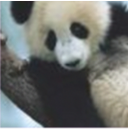
\includegraphics{adv_combined}
            \textbf{\blue{Prediction}}
            \\
            \textbf{Gibbon}
            \\
            99.3\% Confidence
          \end{center}
      \end{column}
    }
    \onslide<+->{
      \begin{column}{0.20\textwidth}
          \begin{center}
            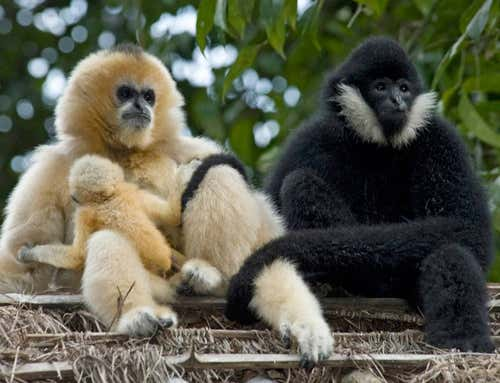
\includegraphics[scale=0.15]{gibbon}
            \textbf{\red{Actual}\\Gibbon}
          \end{center}
      \end{column}
    }
  \end{columns}

\end{frame}

\begin{frame}{$\ell_{p}$ Balls --- Norms First}
  For ${x \in \mathbb{d}}$, the $L_{p}$ norm is:

  \begin{equation}\label{eq:LpNorm}
    \norm{x}_{p} = \left( \sum_{i=1} x_{i}^{p}  \right)^{\frac{1}{p}}
  \end{equation}

  $L_{\infty}$ norm is a special a case:

  \begin{equation}\label{eq:LinftyNorm}
    \norm{x}_{\infty} = \sup_{i} \abs{x_i}
  \end{equation}

  \begin{center}
    \textbf{Note}: $\sup$ equals the $\max$ for a finite set
  \end{center}
\end{frame}

\begin{frame}{$\ell_{p}$ Balls --- Let's Visualize\ldots}
  \begin{definition}
    Given scalar ${\varepsilon > 0}$, the $\ell_{p}$ ball of a point ${x \in \mathbb{R}^{d}}$ is:

    \begin{equation}\label{eq:LpBall}
      \ell_{p}(x) = \setbuild{x + \delta}{\norm{\delta}_{p} \leq \varepsilon}\text{.}
    \end{equation}
  \end{definition}

  \onslide<+->{
    \begin{center}
      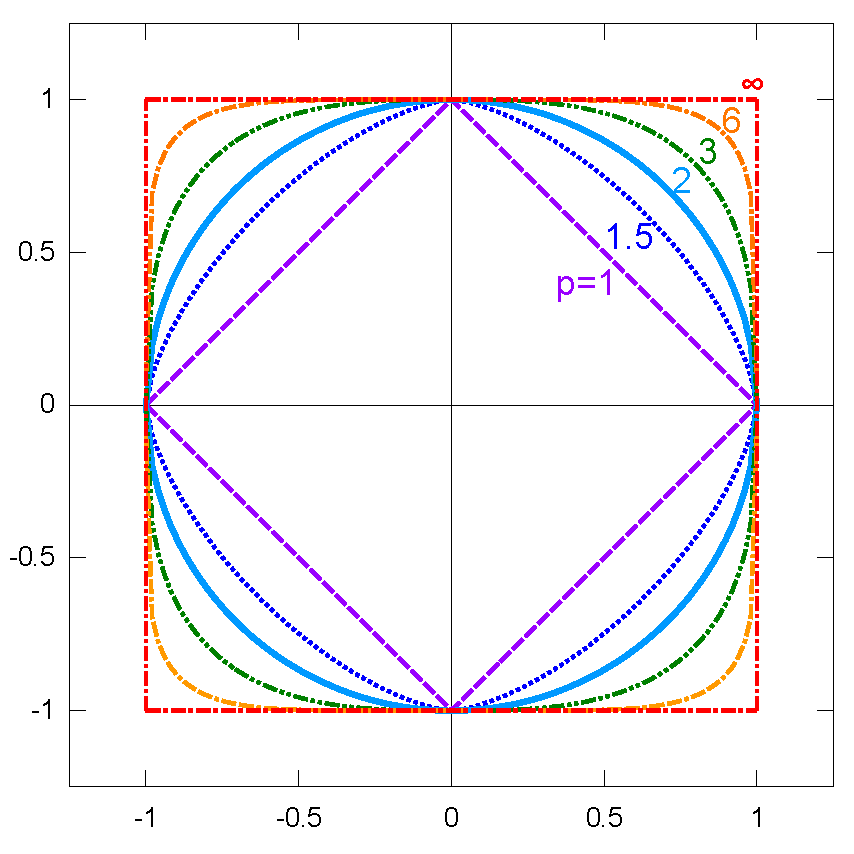
\includegraphics[scale=0.29]{img/lpballs.pdf} \cite{wiki:Lp_space}
    \end{center}
  }
\end{frame}


\begin{frame}{Attack Paradigms}
  \madry\ study adversarial robustness under two different attack paradigms:
  \vfill
  \begin{enumerate}[<+->]
    \item \textbf{Black-Box}: Adversary has no direct access to target network
      \begin{itemize}[<+->]
        \setlength\itemsep{6pt}
        \item \red{Weaker} attack paradigm
        \item Adversary may have \textit{rough} information, e.g.,~model architecture \& training dataset
          \begin{itemize}
            \item \textit{Example}: Transfer attack
          \end{itemize}
        \item Generally \textit{one-shot} attacks
      \end{itemize}
    \vfill
    \item \textbf{White-Box}: Attacker has access to target network's parameter
      \begin{itemize}
        \setlength\itemsep{6pt}
        \item \green{Stronger} attack paradigm
        \item \textit{Examples}: PGD and FGSM (both discussed in this talk)
        \item Enables \textit{iterative} attacks, e.g.,~refined probing
      \end{itemize}
  \end{enumerate}
\end{frame}


\begin{frame}{Nomenclature}
  \onslide<+->{Quite standard and used throughout this talk.}  \onslide<+->{\textit{If you have a question,} \textbf{ask now!}}

  \begin{itemize}[<+->]
    \setlength{\itemsep}{6pt}
    \item ${\X \in \domainX}$: feature values
    \item ${\y \in \domainY}$: Ground truth (true) label
    \item $\func{\distr}{\domainX \times \domainY}{\mathbb{R}_{{\geq}0}}$: Underlying sample data probability distribution s.t.\ ${(\X,\y) \sim \distr}$

    \vspace{6pt}
    \item ${\params \in \domainP}$: Model (neural network) parameters

    \vspace{6pt}
    \item ${\sPerturb \subseteq \domainX}$: Set of allowed (adversarial) perturbations can be applied to any~$\X$
    \item ${\perturb \in \sPerturb}$: (Adversarial) perturbation s.t.
      \begin{equation}\label{eq:AdversarialX}
        \X^{\text{adv}} = x + \delta
      \end{equation}

    \vspace{6pt}
    \item $\mathbb{E}_{x \in \mathcal{X}}\sbrack{f(x)}$: Expected value (weighted mean) of $f(x)$ for all ${x \in \mathcal{X}}$
  \end{itemize}
\end{frame}


\begin{frame}{Nomenclature}
  \begin{itemize}
    \item ${\X \in \mathbb{R}^{d}}$: Training example feature values
    \item ${\y \in \sbrack{k}}$: Training example label

    \item $\params$: Model parameters

    \item $\distr$: Underlying sample data distribution s.t.\ ${(\X,\y) \sim \distr}$
    \item ${\sPerturb \subseteq \mathbb{R}^d}$: Set of allowed (adversarial) perturbations can be applied to any~$\X$
    % \item $\sgn(x) =  \begin{cases}
    %                     1   & x > 0 \\
    %                     0   & x = 0 \\
    %                     -1  & x < 0
    %                   \end{cases}\text{.}$
  \end{itemize}
\end{frame}

\begin{frame}{Fast Gradient Sign Method}
  Simple ``single-step-size'' approach for generating adversarial examples~\cite{Goodfellow:2014}
  \vfill
  Formally:
  \begin{itemize}
    \item $\X$
  \end{itemize}
\end{frame}

\begin{frame}{Projected Gradient Descent}
  \onslide<+->{
    \begin{definition}
      A \textit{\green{projection}} of a point~$y$ onto a set~$X$ is defined as:

      \[ \Pi_{X}(y) = \argmin_{x \in X} \norm{x-y}^{2}_{2}\text{.}  \]
    \end{definition}
  }
  \vfill
  \onslide<+->{
    \begin{definition}
      \textit{\green{Project gradient descent}} (PGD) is a multi-step scheme used to construct adversarial examples.
    \end{definition}
  }
  \onslide<+->{
    \begin{equation}\label{eq:PGD}
      \X^{(t+1)} = \Pi_{x+\sPerturb} \left( \X^{(t)} + \alpha \sgn \left( \nabla_{\X} \loss \left( \X, \y; \theta \right)  \right) \right)
    \end{equation}
  }
\end{frame}

\begin{frame}[allowframebreaks]
  {\tiny
    \frametitle{References}
    \bibliographystyle{ieeetr}
    \bibliography{bib/references.bib}
  }
\end{frame}

\end{document}
